%%=============================================================================
%% LaTeX sjabloon voor bachelorproef, HoGent Bedrijf en Organisatie
%% Opleiding Toegepaste Informatica
%%=============================================================================

\documentclass[fleqn,a4paper,12pt]{book}

%%=============================================================================
%% LaTeX sjabloon voor de bachelorproef, HoGent Bedrijf en Organisatie
%% Opleiding toegepaste informatica
%%
%% Structuur en algemene vormgeving. Meestal hoef je hier niets te wijzigen.
%%
%% Vormgeving gebaseerd op "The Legrand Orange Book", version 2.0 (9/2/15)
%% door Mathias Legrand (legrand.mathias@gmail.com) met aanpassingen door
%% Vel (vel@latextemplates.com). Het oorspronkelijke template is te vinden op
%% http://www.LaTeXTemplates.com
%%
%% Aanpassingen voor HoGent toegepaste informatica:
%%   Bert Van Vreckem <bert.vanvreckem@hogent.be>
%% Licentie:
%%   CC BY-NC-SA 3.0 (http://creativecommons.org/licenses/by-nc-sa/3.0/)
%%=============================================================================

%%-----------------------------------------------------------------------------
%% Packages
%%-----------------------------------------------------------------------------

\usepackage[top=3cm,bottom=3cm,left=3cm,right=3cm,headsep=10pt,a4paper]{geometry} % Page margins
\usepackage[utf8]{inputenc}  % Accenten gebruiken in tekst (vb. é ipv \'e)
\usepackage{amsfonts}        % AMS math packages: extra wiskundige
\usepackage{amsmath}         %   symbolen (o.a. getallen-
\usepackage{amssymb}         %   verzamelingen N, R, Z, Q, etc.)
\usepackage[english,dutch]{babel}    % Taalinstellingen: woordsplitsingen,
                             %  commando's voor speciale karakters
                             %  ("dutch" voor NL)
\usepackage{iflang}
\usepackage{eurosym}         % Euro-symbool €
\usepackage{geometry}
\usepackage{graphicx}        % Invoegen van tekeningen
\graphicspath{{img/}}       % Specifies the directory where pictures are stored
\usepackage{tikz}            % Required for drawing custom shapes
\usepackage[pdftex,bookmarks=true]{hyperref}
                             % PDF krijgt klikbare links & verwijzingen,
                             %  inhoudstafel
\usepackage{enumitem}        % Customize lists
\setlist{nolistsep}         % Reduce spacing between list items
\usepackage{listings}        % Broncode mooi opmaken
\usepackage{multirow}        % Tekst over verschillende cellen in tabellen
\usepackage{rotating}        % Tabellen en figuren roteren

\usepackage{booktabs}        % Required for nicer horizontal rules in tables

\usepackage{xcolor}          % Required for specifying colors by name
\definecolor{maincolor}{RGB}{0,147,208} % Define the main color used for
                             % highlighting throughout the book
                             % 0, 147, 208 = officiële kleur HoGent FBO

% Paragraph style: no indent, add space between paragraphs
\setlength{\parindent}{0em}
\setlength{\parskip}{1em}

\usepackage{etoolbox}
\usepackage{titling} % Macros for title, author, etc
\usepackage{lipsum}          % Voor vultekst (lorem ipsum)

\usepackage{cleveref}        % Reference labels by name
\usepackage[acronym]{glossaries}

\usepackage{tabularx}
\usepackage{booktabs}
\usepackage{makecell}

\usepackage{float,lscape}
\usepackage{pdflscape}

% Table style
\renewcommand\theadalign{bc}
\renewcommand\theadfont{\bfseries}
\renewcommand\theadgape{\Gape[4pt]}
\renewcommand\cellgape{\Gape[4pt]}
\renewcommand{\arraystretch}{2}

% TODOs
\newcommand{\TODO}{}

%----------------------------------------------------------------------------------------
%	FONTS
%----------------------------------------------------------------------------------------

\usepackage{avant} % Use the Avantgarde font for headings
%\usepackage{times} % Use the Times font for headings
\usepackage{mathptmx} % Use the Adobe Times Roman as the default text font together with math symbols from the Sym­bol, Chancery and Com­puter Modern fonts

\usepackage{microtype} % Slightly tweak font spacing for aesthetics
\usepackage[utf8]{inputenc} % Required for including letters with accents
\usepackage[T1]{fontenc} % Use 8-bit encoding that has 256 glyphs

%------------------------------------------------------------------------------
%	TITLE PAGE
%------------------------------------------------------------------------------

\newcommand{\inserttitlepage}{%
\begin{titlepage}
  \newgeometry{top=2cm,bottom=1.5cm,left=1.5cm,right=1.5cm}
  \begin{center}

    \begingroup
    \rmfamily
    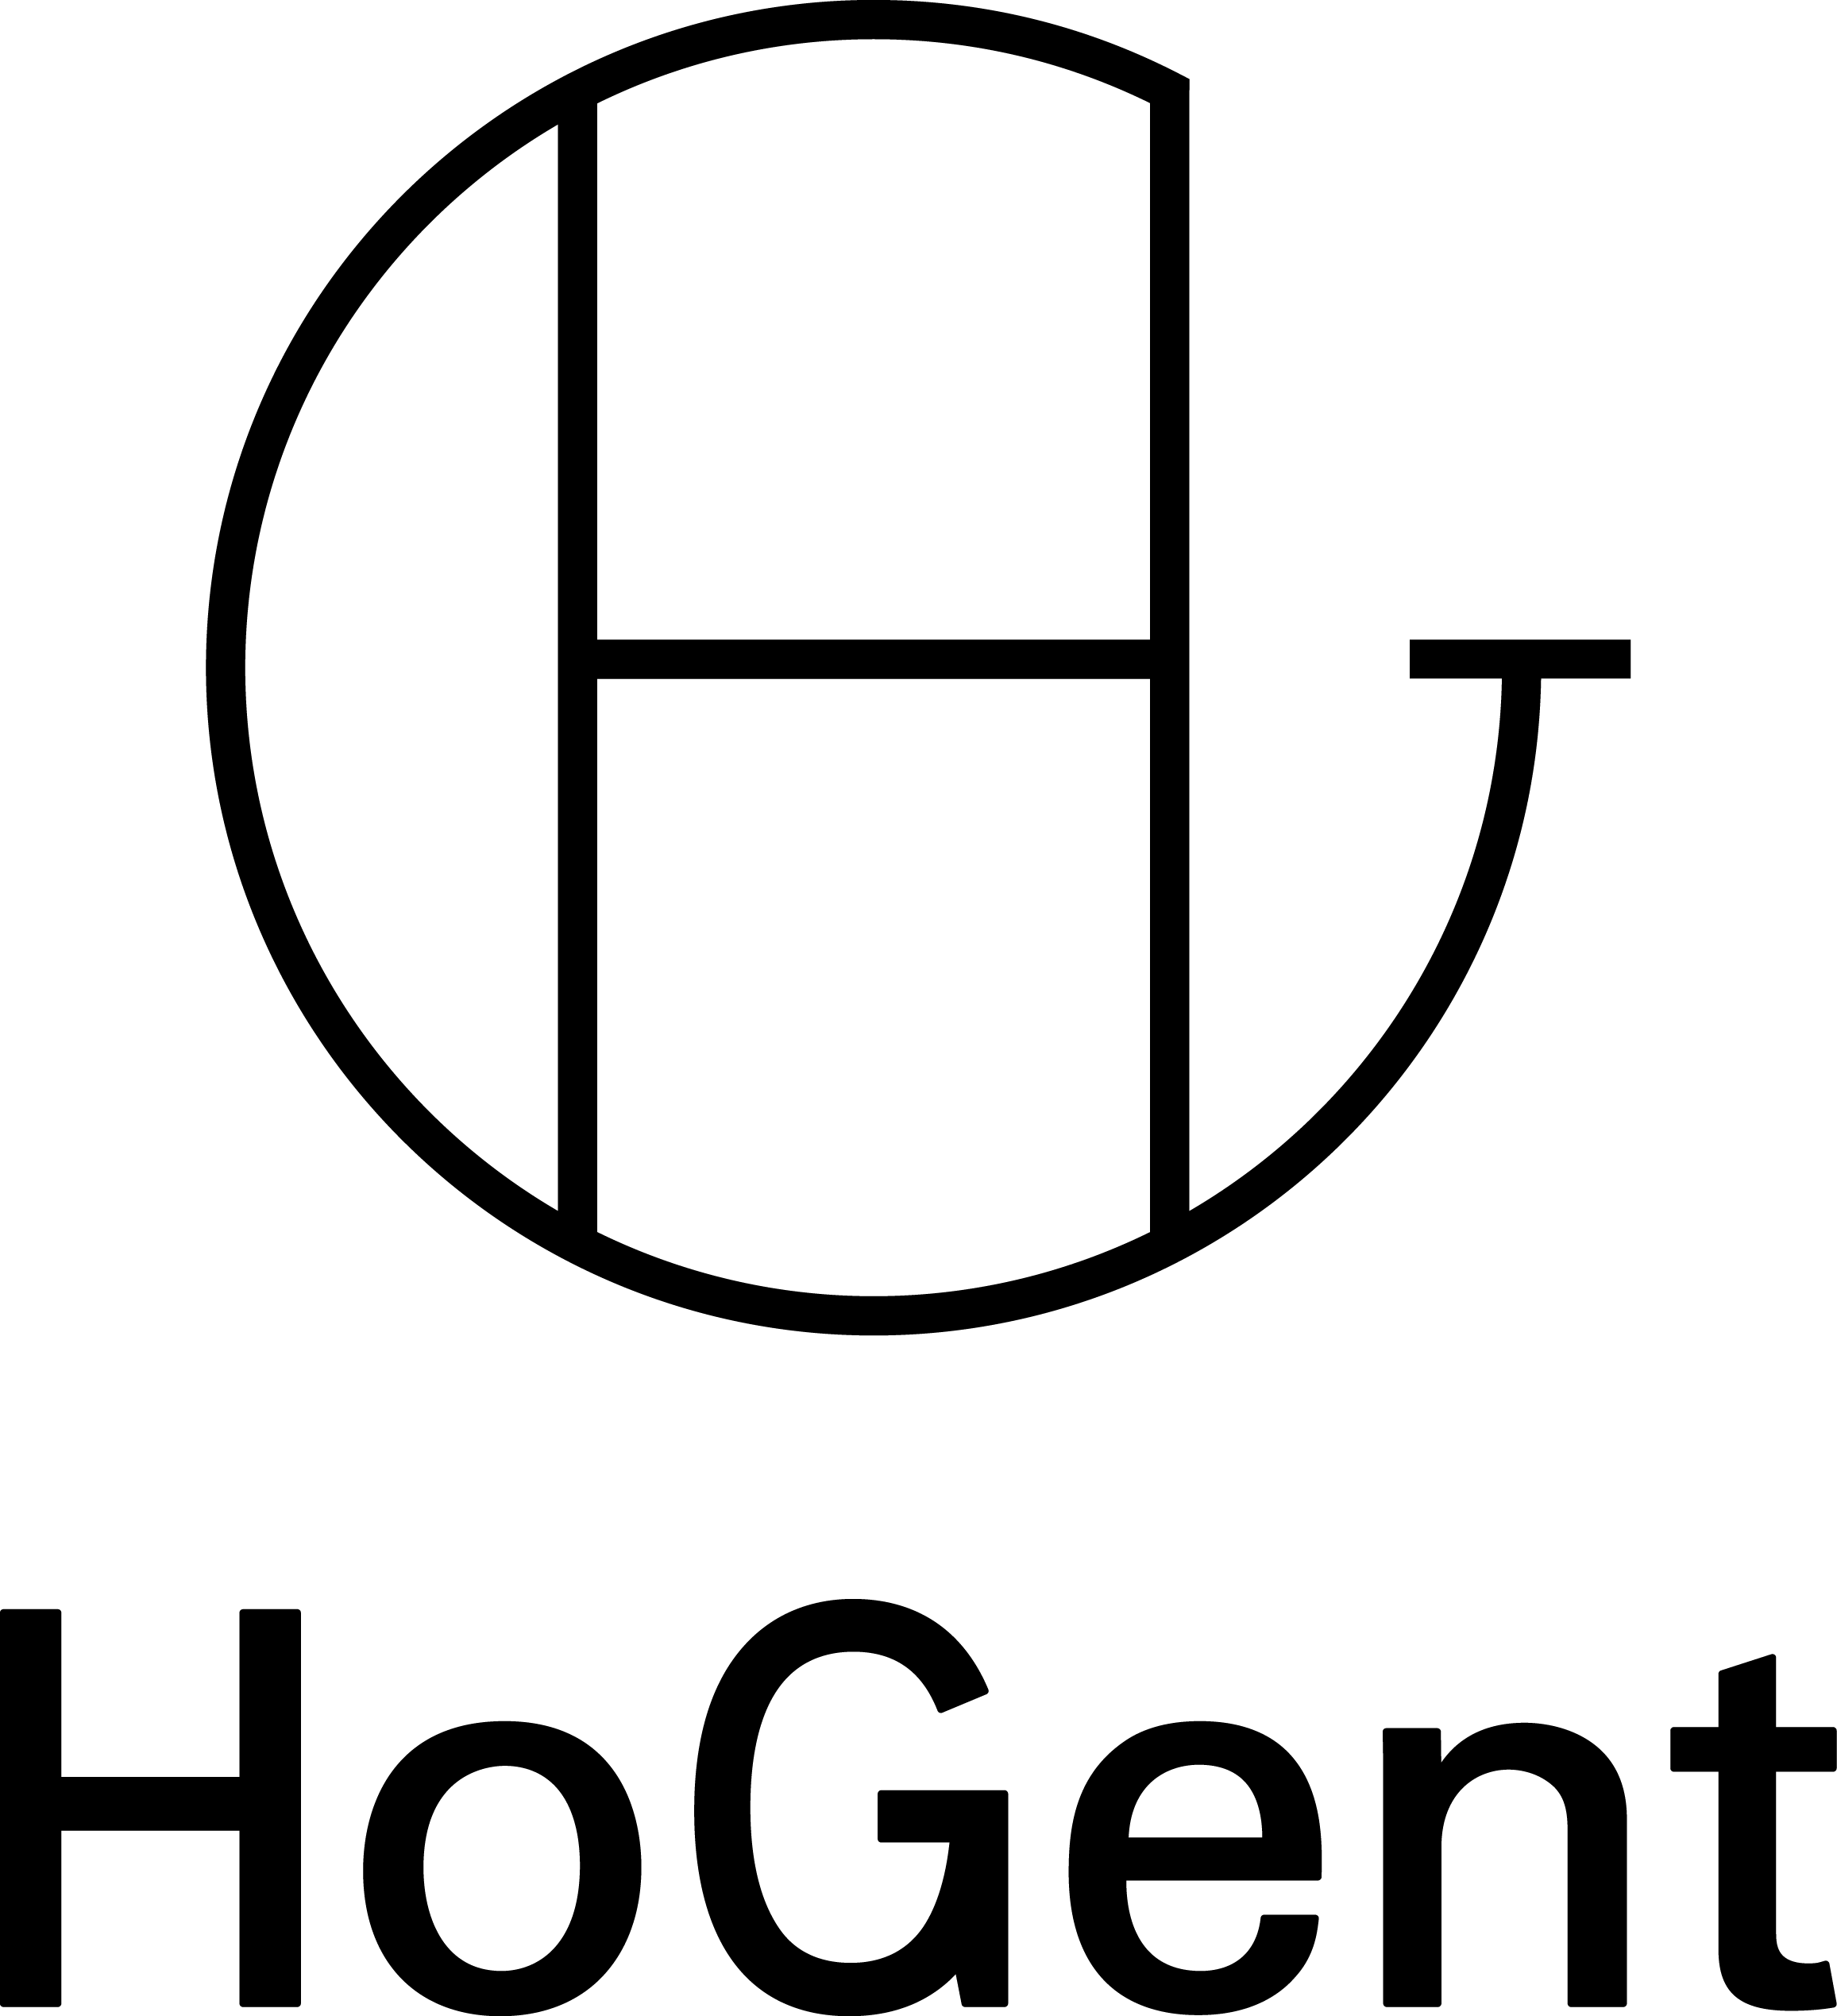
\includegraphics[width=2.5cm]{img/HG-beeldmerk-woordmerk}\\[.5cm]
    Faculteit Bedrijf en Organisatie\\[3cm]
    \titel
    \vfill
    \student\\[3.5cm]
    Scriptie voorgedragen tot het bekomen van de graad van\\professionele bachelor in de toegepaste informatica\\[2cm]
    Promotor:\\
    \promotor\\
    \ifdefempty{\copromotor}{\vspace{2.5cm}}{Co-promotor:\\\copromotor\\[2.5cm]}
    Instelling: \instelling\\[.5cm]
    Academiejaar: \academiejaar\\[.5cm]
    \ifcase \examenperiode \or Eerste \or Tweede \else Derde \fi examenperiode
    \endgroup

  \end{center}
  \restoregeometry
\end{titlepage}
  \emptypage
\begin{titlepage}
  \newgeometry{top=5.35cm,bottom=1.5cm,left=1.5cm,right=1.5cm}
  \begin{center}

    \begingroup
    \rmfamily
    \IfLanguageName{dutch}{Faculteit Bedrijf en Organisatie}{Faculty of Business and Information Management}\\[3cm]
    \titel
    \vfill
    \student\\[3.5cm]
    \IfLanguageName{dutch}{Scriptie voorgedragen tot het bekomen van de graad van\\professionele bachelor in de toegepaste informatica}{Thesis submitted in partial fulfilment of the requirements for the degree of\\professional bachelor of applied computer science}\\[2cm]
    Promotor:\\
    \promotor\\
    \ifdefempty{\copromotor}{\vspace{2.5cm}}{Co-promotor:\\\copromotor\\[2.5cm]}
    \IfLanguageName{dutch}{Instelling}{Institution}: \instelling\\[.5cm]
    \IfLanguageName{dutch}{Academiejaar}{Academic year}: \academiejaar\\[.5cm]
    \IfLanguageName{dutch}{%
    \ifcase \examenperiode \or Eerste \or Tweede \else Derde \fi examenperiode}{%
    \ifcase \examenperiode \or First \or Second \else Third \fi examination period}
    \endgroup

  \end{center}
  \restoregeometry
\end{titlepage}
}

%----------------------------------------------------------------------------------------
%	BIBLIOGRAPHY AND INDEX
%----------------------------------------------------------------------------------------

\usepackage[style=apa,backend=biber]{biblatex}
\usepackage{csquotes}
\DeclareLanguageMapping{dutch}{dutch-apa}
\addbibresource{bibliography.bib} % BibTeX bibliography file
\addbibresource{../proposal/biblio.bib}
\defbibheading{bibempty}{}

\usepackage{calc} % For simpler calculation - used for spacing the index letter headings correctly
\usepackage{makeidx} % Required to make an index
\makeindex % Tells LaTeX to create the files required for indexing

%----------------------------------------------------------------------------------------
%	MAIN TABLE OF CONTENTS
%----------------------------------------------------------------------------------------

\usepackage{titletoc} % Required for manipulating the table of contents

\contentsmargin{0cm} % Removes the default margin

% Part text styling
\titlecontents{part}[0cm]
{\addvspace{20pt}\centering\large\bfseries}
{}
{}
{}

% Chapter text styling
\titlecontents{chapter}[1.25cm] % Indentation
{\addvspace{12pt}\large\sffamily\bfseries} % Spacing and font options for chapters
{\color{maincolor!60}\contentslabel[\Large\thecontentslabel]{1.25cm}\color{maincolor}} % Chapter number
{\color{maincolor}}
{\color{maincolor!60}\normalsize\;\titlerule*[.5pc]{.}\;\thecontentspage} % Page number

% Section text styling
\titlecontents{section}[1.25cm] % Indentation
{\addvspace{3pt}\sffamily\bfseries} % Spacing and font options for sections
{\contentslabel[\thecontentslabel]{1.25cm}} % Section number
{}
{\hfill\color{black}\thecontentspage} % Page number
[]

% Subsection text styling
\titlecontents{subsection}[1.25cm] % Indentation
{\addvspace{1pt}\sffamily\small} % Spacing and font options for subsections
{\contentslabel[\thecontentslabel]{1.25cm}} % Subsection number
{}
{\ \titlerule*[.5pc]{.}\;\thecontentspage} % Page number
[]

% Glossary and list of abbreviations
\newglossaryentry{clustering}{
  name = $clustering$,
  description = {The horizontal scaling ability of a distributed data store over multiple hosts and the interactions within the network between the cluster nodes},
}

\newglossaryentry{datastore}{
  name = $data store$,
  description = A repository of persistently stored and managed collections of data,
}

\newglossaryentry{database}{
  name = $database$,
  description = A data store managed by an database management system,
}

\newglossaryentry{dbms}{
  name = $database management system$,
  description = {Software that manages storage, querying and manipulation of data in a database},
}

\newglossaryentry{cap-theorem}{
  name = $CAP theorem$,
  description = {The proposition that states that a distributed database cannot provide more than two out of three of the CAP guarantees: Consistency, Availability, Partition tolerance},
}

\newglossaryentry{impedance-mismatch}{
name = $Impedance Mismatch$,
description = {The difference between the relational model and the data structures provided by the programming language},
}

\newglossaryentry{newsql}{
  name = $NewSQL$,
  description = {Classification of modern relational database that aims to provide solutions to the scalability and flexibility similar to NoSQL systems, while still maintaining ACID guarantees},
}

\newglossaryentry{nosql}{
  name = $NoSQL$,
  description = {Not Only SQL, classification of modern non-relational database that focuses on horizontal scalability and flexibility in data model},
}

\newglossaryentry{polyglot-persistence}{
  name = $Polyglot Persistence$,
  description = {The practice of using multiple databases to store different types of information},
}

\newglossaryentry{restful}{
  name = $RESTful$,
  description = {Conforming to the REST architecture},
}

\newglossaryentry{sharding}{
  name = $sharding$,
  description = {Distributing of the dataset within a distributed data store, based on certain criteria within the data itself},
}

\newacronym{rdbms}{RDBMS}{Relational Database Management System}
\newacronym{erd}{ERD}{Entity Relationship Diagram}
\newacronym{acid}{ACID}{Atomicity, Consistency, Isolation, Durability}
\newacronym{base}{BASE}{Basically Available, Soft state, Eventual consistency}
\newacronym{rdf}{RDF}{Resource Description Framework}
\newacronym{oltp}{OLTP}{Online Transaction Processing}

\makeglossaries

% List of figures
\titlecontents{figure}[0em]
{\addvspace{-5pt}\sffamily}
{\thecontentslabel\hspace*{1em}}
{}
{\ \titlerule*[.5pc]{.}\;\thecontentspage}
[]

% List of tables
\titlecontents{table}[0em]
{\addvspace{-5pt}\sffamily}
{\thecontentslabel\hspace*{1em}}
{}
{\ \titlerule*[.5pc]{.}\;\thecontentspage}
[]

%----------------------------------------------------------------------------------------
%	MINI TABLE OF CONTENTS IN PART HEADS
%----------------------------------------------------------------------------------------

% Chapter text styling
\titlecontents{lchapter}[0em] % Indenting
{\addvspace{15pt}\large\sffamily\bfseries} % Spacing and font options for chapters
{\color{maincolor}\contentslabel[\Large\thecontentslabel]{1.25cm}\color{maincolor}} % Chapter number
{}
{\color{maincolor}\normalsize\sffamily\bfseries\;\titlerule*[.5pc]{.}\;\thecontentspage} % Page number

% Section text styling
\titlecontents{lsection}[0em] % Indenting
{\sffamily\small} % Spacing and font options for sections
{\contentslabel[\thecontentslabel]{1.25cm}} % Section number
{}
{}

% Subsection text styling
\titlecontents{lsubsection}[.5em] % Indentation
{\normalfont\footnotesize\sffamily} % Font settings
{}
{}
{}

%----------------------------------------------------------------------------------------
%	PAGE HEADERS
%----------------------------------------------------------------------------------------

\usepackage{fancyhdr} % Required for header and footer configuration

\pagestyle{fancy}
\renewcommand{\chaptermark}[1]{\markboth{\sffamily\normalsize\bfseries\chaptername\ \thechapter.\ #1}{}} % Chapter text font settings
\renewcommand{\sectionmark}[1]{\markright{\sffamily\normalsize\thesection\hspace{5pt}#1}{}} % Section text font settings
\fancyhf{} \fancyhead[LE,RO]{\sffamily\normalsize\thepage} % Font setting for the page number in the header
\fancyhead[LO]{\rightmark} % Print the nearest section name on the left side of odd pages
\fancyhead[RE]{\leftmark} % Print the current chapter name on the right side of even pages
\renewcommand{\headrulewidth}{0.5pt} % Width of the rule under the header
\addtolength{\headheight}{2.5pt} % Increase the spacing around the header slightly
\renewcommand{\footrulewidth}{0pt} % Removes the rule in the footer
\fancypagestyle{plain}{\fancyhead{}\renewcommand{\headrulewidth}{0pt}} % Style for when a plain pagestyle is specified

% Removes the header from odd empty pages at the end of chapters
\makeatletter
\renewcommand{\cleardoublepage}{
\clearpage\ifodd\c@page\else
\hbox{}
\vspace*{\fill}
\thispagestyle{empty}
\newpage
\fi}

%----------------------------------------------------------------------------------------
%	THEOREM STYLES
%----------------------------------------------------------------------------------------

\usepackage{amsmath,amsfonts,amssymb,amsthm} % For math equations, theorems, symbols, etc

\newcommand{\intoo}[2]{\mathopen{]}#1\,;#2\mathclose{[}}
\newcommand{\ud}{\mathop{\mathrm{{}d}}\mathopen{}}
\newcommand{\intff}[2]{\mathopen{[}#1\,;#2\mathclose{]}}
\newtheorem{notation}{Notation}[chapter]

% Boxed/framed environments
\newtheoremstyle{maincolornumbox}% % Theorem style name
{0pt}% Space above
{0pt}% Space below
{\normalfont}% % Body font
{}% Indent amount
{\small\bf\sffamily\color{maincolor}}% % Theorem head font
{\;}% Punctuation after theorem head
{0.25em}% Space after theorem head
{\small\sffamily\color{maincolor}\thmname{#1}\nobreakspace\thmnumber{\@ifnotempty{#1}{}\@upn{#2}}% Theorem text (e.g. Theorem 2.1)
\thmnote{\nobreakspace\the\thm@notefont\sffamily\bfseries\color{black}---\nobreakspace#3.}} % Optional theorem note
\renewcommand{\qedsymbol}{$\blacksquare$}% Optional qed square

\newtheoremstyle{blacknumex}% Theorem style name
{5pt}% Space above
{5pt}% Space below
{\normalfont}% Body font
{} % Indent amount
{\small\bf\sffamily}% Theorem head font
{\;}% Punctuation after theorem head
{0.25em}% Space after theorem head
{\small\sffamily{\tiny\ensuremath{\blacksquare}}\nobreakspace\thmname{#1}\nobreakspace\thmnumber{\@ifnotempty{#1}{}\@upn{#2}}% Theorem text (e.g. Theorem 2.1)
\thmnote{\nobreakspace\the\thm@notefont\sffamily\bfseries---\nobreakspace#3.}}% Optional theorem note

\newtheoremstyle{blacknumbox} % Theorem style name
{0pt}% Space above
{0pt}% Space below
{\normalfont}% Body font
{}% Indent amount
{\small\bf\sffamily}% Theorem head font
{\;}% Punctuation after theorem head
{0.25em}% Space after theorem head
{\small\sffamily\thmname{#1}\nobreakspace\thmnumber{\@ifnotempty{#1}{}\@upn{#2}}% Theorem text (e.g. Theorem 2.1)
\thmnote{\nobreakspace\the\thm@notefont\sffamily\bfseries---\nobreakspace#3.}}% Optional theorem note

% Non-boxed/non-framed environments
\newtheoremstyle{maincolornum}% % Theorem style name
{5pt}% Space above
{5pt}% Space below
{\normalfont}% % Body font
{}% Indent amount
{\small\bf\sffamily\color{maincolor}}% % Theorem head font
{\;}% Punctuation after theorem head
{0.25em}% Space after theorem head
{\small\sffamily\color{maincolor}\thmname{#1}\nobreakspace\thmnumber{\@ifnotempty{#1}{}\@upn{#2}}% Theorem text (e.g. Theorem 2.1)
\thmnote{\nobreakspace\the\thm@notefont\sffamily\bfseries\color{black}---\nobreakspace#3.}} % Optional theorem note
\renewcommand{\qedsymbol}{$\blacksquare$}% Optional qed square
\makeatother

% Defines the theorem text style for each type of theorem to one of the three styles above
\newcounter{dummy}
\numberwithin{dummy}{section}
\theoremstyle{maincolornumbox}
\newtheorem{theoremeT}[dummy]{Theorem}
\newtheorem{problem}{Problem}[chapter]
\newtheorem{exerciseT}{Exercise}[chapter]
\theoremstyle{blacknumex}
\newtheorem{exampleT}{Example}[chapter]
\theoremstyle{blacknumbox}
\newtheorem{vocabulary}{Vocabulary}[chapter]
\newtheorem{definitionT}{Definition}[section]
\newtheorem{corollaryT}[dummy]{Corollary}
\theoremstyle{maincolornum}
\newtheorem{proposition}[dummy]{Proposition}

%----------------------------------------------------------------------------------------
%	DEFINITION OF COLORED BOXES
%----------------------------------------------------------------------------------------

\RequirePackage[framemethod=default]{mdframed} % Required for creating the theorem, definition, exercise and corollary boxes

% Theorem box
\newmdenv[skipabove=7pt,
skipbelow=7pt,
backgroundcolor=black!5,
linecolor=maincolor,
innerleftmargin=5pt,
innerrightmargin=5pt,
innertopmargin=5pt,
leftmargin=0cm,
rightmargin=0cm,
innerbottommargin=5pt]{tBox}

% Exercise box
\newmdenv[skipabove=7pt,
skipbelow=7pt,
rightline=false,
leftline=true,
topline=false,
bottomline=false,
backgroundcolor=maincolor!10,
linecolor=maincolor,
innerleftmargin=5pt,
innerrightmargin=5pt,
innertopmargin=5pt,
innerbottommargin=5pt,
leftmargin=0cm,
rightmargin=0cm,
linewidth=4pt]{eBox}

% Definition box
\newmdenv[skipabove=7pt,
skipbelow=7pt,
rightline=false,
leftline=true,
topline=false,
bottomline=false,
linecolor=maincolor,
innerleftmargin=5pt,
innerrightmargin=5pt,
innertopmargin=0pt,
leftmargin=0cm,
rightmargin=0cm,
linewidth=4pt,
innerbottommargin=0pt]{dBox}

% Corollary box
\newmdenv[skipabove=7pt,
skipbelow=7pt,
rightline=false,
leftline=true,
topline=false,
bottomline=false,
linecolor=gray,
backgroundcolor=black!5,
innerleftmargin=5pt,
innerrightmargin=5pt,
innertopmargin=5pt,
leftmargin=0cm,
rightmargin=0cm,
linewidth=4pt,
innerbottommargin=5pt]{cBox}

% Creates an environment for each type of theorem and assigns it a theorem text style from the "Theorem Styles" section above and a colored box from above
\newenvironment{theorem}{\begin{tBox}\begin{theoremeT}}{\end{theoremeT}\end{tBox}}
\newenvironment{exercise}{\begin{eBox}\begin{exerciseT}}{\hfill{\color{maincolor}\tiny\ensuremath{\blacksquare}}\end{exerciseT}\end{eBox}}
\newenvironment{definition}{\begin{dBox}\begin{definitionT}}{\end{definitionT}\end{dBox}}
\newenvironment{example}{\begin{exampleT}}{\hfill{\tiny\ensuremath{\blacksquare}}\end{exampleT}}
\newenvironment{corollary}{\begin{cBox}\begin{corollaryT}}{\end{corollaryT}\end{cBox}}

%----------------------------------------------------------------------------------------
%	REMARK ENVIRONMENT
%----------------------------------------------------------------------------------------

\newenvironment{remark}{\par\vspace{10pt}\small % Vertical white space above the remark and smaller font size
\begin{list}{}{
\leftmargin=35pt % Indentation on the left
\rightmargin=25pt}\item\ignorespaces % Indentation on the right
\makebox[-2.5pt]{\begin{tikzpicture}[overlay]
\node[draw=maincolor!60,line width=1pt,circle,fill=maincolor!25,font=\sffamily\bfseries,inner sep=2pt,outer sep=0pt] at (-15pt,0pt){\textcolor{maincolor}{R}};\end{tikzpicture}} % Orange R in a circle
\advance\baselineskip -1pt}{\end{list}\vskip5pt} % Tighter line spacing and white space after remark

%----------------------------------------------------------------------------------------
%	SECTION NUMBERING IN THE MARGIN
%----------------------------------------------------------------------------------------

\makeatletter
\renewcommand{\@seccntformat}[1]{\llap{\textcolor{maincolor}{\csname the#1\endcsname}\hspace{1em}}}
\renewcommand{\section}{\@startsection{section}{1}{\z@}
{-4ex \@plus -1ex \@minus -.4ex}
{1ex \@plus.2ex }
{\normalfont\large\sffamily\bfseries}}
\renewcommand{\subsection}{\@startsection {subsection}{2}{\z@}
{-3ex \@plus -0.1ex \@minus -.4ex}
{0.5ex \@plus.2ex }
{\normalfont\sffamily\bfseries}}
\renewcommand{\subsubsection}{\@startsection {subsubsection}{3}{\z@}
{-2ex \@plus -0.1ex \@minus -.2ex}
{.2ex \@plus.2ex }
{\normalfont\small\sffamily\bfseries}}
\renewcommand\paragraph{\@startsection{paragraph}{4}{\z@}
{-2ex \@plus-.2ex \@minus .2ex}
{.1ex}
{\normalfont\small\sffamily\bfseries}}

%----------------------------------------------------------------------------------------
%	PART HEADINGS
%----------------------------------------------------------------------------------------

% numbered part in the table of contents
\newcommand{\@mypartnumtocformat}[2]{%
\setlength\fboxsep{0pt}%
\noindent\colorbox{maincolor!20}{\strut\parbox[c][.7cm]{\ecart}{\color{maincolor!70}\Large\sffamily\bfseries\centering#1}}\hskip\esp\colorbox{maincolor!40}{\strut\parbox[c][.7cm]{\linewidth-\ecart-\esp}{\Large\sffamily\centering#2}}}%
%%%%%%%%%%%%%%%%%%%%%%%%%%%%%%%%%%
% unnumbered part in the table of contents
\newcommand{\@myparttocformat}[1]{%
\setlength\fboxsep{0pt}%
\noindent\colorbox{maincolor!40}{\strut\parbox[c][.7cm]{\linewidth}{\Large\sffamily\centering#1}}}%
%%%%%%%%%%%%%%%%%%%%%%%%%%%%%%%%%%
\newlength\esp
\setlength\esp{4pt}
\newlength\ecart
\setlength\ecart{1.2cm-\esp}
\newcommand{\thepartimage}{}%
\newcommand{\partimage}[1]{\renewcommand{\thepartimage}{#1}}%
\def\@part[#1]#2{%
\ifnum \c@secnumdepth >-2\relax%
\refstepcounter{part}%
\addcontentsline{toc}{part}{\texorpdfstring{\protect\@mypartnumtocformat{\thepart}{#1}}{\partname~\thepart\ ---\ #1}}
\else%
\addcontentsline{toc}{part}{\texorpdfstring{\protect\@myparttocformat{#1}}{#1}}%
\fi%
\startcontents%
\markboth{}{}%
{\thispagestyle{empty}%
\begin{tikzpicture}[remember picture,overlay]%
\node at (current page.north west){\begin{tikzpicture}[remember picture,overlay]%
\fill[maincolor!20](0cm,0cm) rectangle (\paperwidth,-\paperheight);
\node[anchor=north] at (4cm,-3.25cm){\color{maincolor!40}\fontsize{220}{100}\sffamily\bfseries\@Roman\c@part};
\node[anchor=south east] at (\paperwidth-1cm,-\paperheight+1cm){\parbox[t][][t]{8.5cm}{
\printcontents{l}{0}{\setcounter{tocdepth}{1}}%
}};
\node[anchor=north east] at (\paperwidth-1.5cm,-3.25cm){\parbox[t][][t]{15cm}{\strut\raggedleft\color{white}\fontsize{30}{30}\sffamily\bfseries#2}};
\end{tikzpicture}};
\end{tikzpicture}}%
\@endpart}
\def\@spart#1{%
\startcontents%
\phantomsection
{\thispagestyle{empty}%
\begin{tikzpicture}[remember picture,overlay]%
\node at (current page.north west){\begin{tikzpicture}[remember picture,overlay]%
\fill[maincolor!20](0cm,0cm) rectangle (\paperwidth,-\paperheight);
\node[anchor=north east] at (\paperwidth-1.5cm,-3.25cm){\parbox[t][][t]{15cm}{\strut\raggedleft\color{white}\fontsize{30}{30}\sffamily\bfseries#1}};
\end{tikzpicture}};
\end{tikzpicture}}
\addcontentsline{toc}{part}{\texorpdfstring{%
\setlength\fboxsep{0pt}%
\noindent\protect\colorbox{maincolor!40}{\strut\protect\parbox[c][.7cm]{\linewidth}{\Large\sffamily\protect\centering #1\quad\mbox{}}}}{#1}}%
\@endpart}
\def\@endpart{\vfil\newpage
\if@twoside
\if@openright
\null
\thispagestyle{empty}%
\newpage
\fi
\fi
\if@tempswa
\twocolumn
\fi}

%----------------------------------------------------------------------------------------
%	CHAPTER HEADINGS
%----------------------------------------------------------------------------------------

% A switch to conditionally include a picture, implemented by  Christian Hupfer
\newif\ifusechapterimage
\usechapterimagetrue
\newcommand{\thechapterimage}{}%
\newcommand{\chapterimage}[1]{\ifusechapterimage\renewcommand{\thechapterimage}{#1}\fi}%
\def\@makechapterhead#1{%
{\parindent \z@ \raggedright \normalfont
\ifnum \c@secnumdepth >\m@ne
\if@mainmatter
\begin{tikzpicture}[remember picture,overlay]
\node at (current page.north west)
{\begin{tikzpicture}[remember picture,overlay]
\node[anchor=north west,inner sep=0pt] at (0,0) {\ifusechapterimage\includegraphics[width=\paperwidth]{\thechapterimage}\fi};
\draw[anchor=west] (\Gm@lmargin,-9cm) node [line width=2pt,rounded corners=15pt,draw=maincolor,fill=white,fill opacity=0.5,inner sep=15pt]{\strut\makebox[22cm]{}};
\draw[anchor=west] (\Gm@lmargin+.3cm,-9cm) node {\huge\sffamily\bfseries\color{black}\thechapter. #1\strut};
\end{tikzpicture}};
\end{tikzpicture}
\else
\begin{tikzpicture}[remember picture,overlay]
\node at (current page.north west)
{\begin{tikzpicture}[remember picture,overlay]
\node[anchor=north west,inner sep=0pt] at (0,0) {\ifusechapterimage\includegraphics[width=\paperwidth]{\thechapterimage}\fi};
\draw[anchor=west] (\Gm@lmargin,-9cm) node [line width=2pt,rounded corners=15pt,draw=maincolor,fill=white,fill opacity=0.5,inner sep=15pt]{\strut\makebox[22cm]{}};
\draw[anchor=west] (\Gm@lmargin+.3cm,-9cm) node {\huge\sffamily\bfseries\color{black}#1\strut};
\end{tikzpicture}};
\end{tikzpicture}
\fi\fi\par\vspace*{270\p@}}}

%-------------------------------------------

\def\@makeschapterhead#1{%
\begin{tikzpicture}[remember picture,overlay]
\node at (current page.north west)
{\begin{tikzpicture}[remember picture,overlay]
\node[anchor=north west,inner sep=0pt] at (0,0) {\ifusechapterimage\includegraphics[width=\paperwidth]{\thechapterimage}\fi};
\draw[anchor=west] (\Gm@lmargin,-9cm) node [line width=2pt,rounded corners=15pt,draw=maincolor,fill=white,fill opacity=0.5,inner sep=15pt]{\strut\makebox[22cm]{}};
\draw[anchor=west] (\Gm@lmargin+.3cm,-9cm) node {\huge\sffamily\bfseries\color{black}#1\strut};
\end{tikzpicture}};
\end{tikzpicture}
\par\vspace*{270\p@}}
\makeatother

%----------------------------------------------------------------------------------------
%	HYPERLINKS IN THE DOCUMENTS
%----------------------------------------------------------------------------------------

\usepackage{hyperref}
\hypersetup{hidelinks,backref=true,pagebackref=true,hyperindex=true,colorlinks=false,breaklinks=true,urlcolor= maincolor,bookmarks=true,bookmarksopen=false,pdftitle={Title},pdfauthor={Author}}
\usepackage{bookmark}
\bookmarksetup{
open,
numbered,
addtohook={%
\ifnum\bookmarkget{level}=0 % chapter
\bookmarksetup{bold}%
\fi
\ifnum\bookmarkget{level}=-1 % part
\bookmarksetup{color=maincolor,bold}%
\fi
}
}

%----------------------------------------------------------------------------------------
%	Java source code
%----------------------------------------------------------------------------------------

% Commando voor invoegen Java-broncodebestanden (dank aan Niels Corneille)
% Gebruik:
%   \codefragment{source/MijnKlasse.java}{Uitleg bij de code}
%
% Je kan dit aanpassen aan de taal die je zelf het meeste gebruikt in je
% bachelorproef.
\newcommand{\codefragment}[2]{ \lstset{%
  language=java,
  breaklines=true,
  float=th,
  caption={#2},
  basicstyle=\scriptsize,
  frame=single,
  extendedchars=\true
}
\lstinputlisting{#1}}

% Leeg blad
\newcommand{\emptypage}{%
\newpage
\thispagestyle{empty}
\mbox{}
\newpage
}


%%---------- Documenteigenschappen --------------------------------------------
%% TODO: Vul dit aan met je eigen info:

% Je eigen naam
\newcommand{\student}{Florian Dejonckheere}

% De naam van je promotor (lector van de opleiding)
\newcommand{\promotor}{Chantal Teerlinck}

% De naam van je co-promotor. Als je promotor ook je opdrachtgever is en je
% dus ook inhoudelijk begeleidt (en enkel dan!), mag je dit leeg laten.
\newcommand{\copromotor}{}

% Indien je bachelorproef in opdracht van/in samenwerking met een bedrijf of
% externe organisatie geschreven is, geef je hier de naam. Zoniet laat je dit
% zoals het is.
\newcommand{\instelling}{Open Webslides}

% De titel van het rapport/bachelorproef
\newcommand{\titel}{Analysis and Design of an Efficient NoSQL Data Storage Schema for an Interlinked Recent Activity Feed}

% Datum van indienen (gebruik telkens de deadline, ook al geef je eerder af)
\newcommand{\datum}{28 May 2018}

% Academiejaar
\newcommand{\academiejaar}{2017-2018}

% Examenperiode
%  - 1e semester = 1e examenperiode => 1
%  - 2e semester = 2e examenperiode => 2
%  - tweede zit  = 3e examenperiode => 3
\newcommand{\examenperiode}{2}

%%=============================================================================
%% Inhoud document
%%=============================================================================

\begin{document}

%---------- Taalselectie ------------------------------------------------------
% Als je je bachelorproef in het Engels schrijft, haal dan onderstaande regel
% uit commentaar. Let op: de tekst op de voorkaft blijft in het Nederlands, en
% dat is ook de bedoeling!

\selectlanguage{english}

%---------- Titelblad ---------------------------------------------------------
\inserttitlepage

%---------- Samenvatting, voorwoord -------------------------------------------
\usechapterimagefalse
%%=============================================================================
%% Preface
%%=============================================================================

\chapter*{Preface}
\label{ch:preface}

The idea for this research originally comes from the Open Webslides project and its many little side activities in development.
One of the things that has always fascinated me was how the platform would handle a massive influx of users, and specifically how it would relate to the non-critical data storage of the news items in the \textit{Recent Activity} feed.
I wanted to find out how a NoSQL data store would be integrated into the flow of data, and what kind of data store would be the most efficient, scalable solution for this problem.
My interest in this problem was also piqued by using the Neo4j graph database in a personal project, and how the data of the Open Webslides project would fit into the graph theoretical model as opposed to the relational model.
Digging into this subject while still maintaining my vision on the Ruby on Rails implementation in the platform allowed me to let the question bloom into this research paper.

This thesis was in part achieved by the support of Chantal Teerlinck, my promotor, who has given me many tips and tricks, and provided a framework for conducting a proper research.
Guy De Tr\'e, my co-promotor, also had an important influence on decisions taken in the research and development phase, being a person who is immersed in the academic world of relational and non-relational database management systems.
Finally, my friends and family also deserve recognition for helping me accomplish this paper, which is the culmination of three years higher education in a fast-moving and innovative field.

\begin {flushright}
  Florian Dejonckheere, Ghent, May 2018
\end {flushright}

%%=============================================================================
%% Summary
%%=============================================================================

% Deze aspecten moeten zeker aan bod komen:
% - Context: waarom is dit werk belangrijk?
% - Nood: waarom moest dit onderzocht worden?
% - Taak: wat heb je precies gedaan?
% - Object: wat staat in dit document geschreven?
% - Resultaat: wat was het resultaat?
% - Conclusie: wat is/zijn de belangrijkste conclusie(s)?
% - Perspectief: blijven er nog vragen open die in de toekomst nog kunnen
%    onderzocht worden? Wat is een mogelijk vervolg voor jouw onderzoek?
%
% LET OP! Een samenvatting is GEEN voorwoord!

%%---------- Nederlandse samenvatting -----------------------------------------
%
% TODO: Als je je bachelorproef in het Engels schrijft, moet je eerst een
% Nederlandse samenvatting invoegen. Haal daarvoor onderstaande code uit
% commentaar.
% Wie zijn bachelorproef in het Nederlands schrijft, kan dit negeren, de inhoud
% wordt niet in het document ingevoegd.

\IfLanguageName{english}{%
\selectlanguage{dutch}
\chapter*{Samenvatting}

De opkomst van grootschalige, dynamische web applicaties heeft geleid tot een enorme toename in de behoefte voor performante database systemen om de overvloed van informatie gegenereerd door gebruikersactiviteit op te slaan.
Het antwoord van de industry op dit probleem is de NoSQL beweging, die beschikbaarheid and schaalbaarheid verkiest over traditionele belangen zoals data consistentie en betrouwbaarheid.
Een belangrijker wordende vraag voor onderzoekers en ontwikkelaars in het vakdomein is hoe de opslag van deze informatie efficient kan gebeuren, om de performantie van de queries te maximaliseren, toegepast op de relevante use case en inherente structuur van de betrokken data.

Deze thesis duikt in de wereld van NoSQL en niet-relationele data modeling door middel van een vergelijkende studie van diverse NoSQL data store categorie\"{e}n en leveranciers.
De \textit{Recent Activity feed} van het Open Webslides project wordt gebruikt als case study.
Een vergelijkende studie voor elk van de \TODO{vijf} categorie\"{e}n van NoSQL data stores wordt naar voren geschoven, waarbij factoren relevant voor de use case besproken worden.
Vervolgens worden twee logische datamodellen voor document en graph data stores opgesteld, samen met drie bijbehorende implementaties voor de MongoDB, CouchDB en Neo4j data stores.

Het onderzoek concludeert dat document stores de meest effici\"{e}nte oplossing bieden onder de vergeleken categorie\"{e}n.
De NoSQL data stores worden in het Open Webslides platform gebruikt complementair aan een relationele database, gebruik makend van \textit{polyglot persistence} om een performante en schaalbare applicatie te verkrijgen.

De NoSQL implementaties ontwikkeld in deze thesis zullen bekwame en krachtige oplossingen bieden voor het probleem voorgesteld in de case study.
Er zijn echter ook veel mogelijkheden om de grenzen van dit onderzoek te overstijgen boven de aanvankelijke use case, en verdere contributies aan het vakdomein te leveren.


\selectlanguage{english}
}{}

%%---------- Samenvatting -----------------------------------------------------
% De samenvatting in de hoofdtaal van het document

\chapter*{\IfLanguageName{dutch}{Samenvatting}{Abstract}}

The advent of large scale, dynamic web applications has led to a massive increase in the need for performant database systems to store the deluge of information generated by user activity.
The industry's answer to this problem is the NoSQL movement, which prioritizes availability and scalability over traditional concerns such as data consistency and reliability.
An increasingly interesting question for researchers and developers in the field is how to store this data in order to maximize the query performance, considering the use case and the inherent structure of the data involved.

This paper dives into the world of NoSQL and non-relational data modeling, comparing and examining the different NoSQL data store types and vendors.
In this comparative study, the \textit{Recent Activity} feed of the Open Webslides platform is used as a case study.
For the \TODO{five} categories of NoSQL data stores, a comparative study is presented in which aspects relevant to the use case are compared.
Subsequently, two logical data models for document and graph data stores are presented, along with three corresponding implementations for the MongoDB, CouchDB and Neo4j data stores.

The research concluded that document stores are the most efficient data stores among the solutions considered.
The NoSQL data stores are to be used complementary with a relational database, leveraging polyglot persistence to achieve a performant and scalable web application.

The NoSQL implementations developed in this thesis will provide capable and powerful solutions for the problem presented in the case study.
However, it was found that there are many opportunities to extend this research beyond the initial use case to allow additional contributions to the field.


%---------- Inhoudstafel ------------------------------------------------------
\pagestyle{empty} % No headers
\tableofcontents % Print the table of contents itself
\cleardoublepage % Forces the first chapter to start on an odd page so it's on the right
\pagestyle{fancy} % Print headers again

%---------- List of abbreviations and glossary --------------------------------

\printglossary
\printglossary[type=\acronymtype,title={List of abbreviations}]


%---------- Lijst figuren, afkortingen, ... -----------------------------------

% Indien gewenst kan je hier een lijst van figuren/tabellen opgeven. Geef in
% dat geval je figuren/tabellen altijd een korte beschrijving:
%
%  \caption[korte beschrijving]{uitgebreide beschrijving}

\listoffigures
\listoftables

% Als je een lijst van afkortingen of termen wil toevoegen, dan hoort die
% hier thuis. Gebruik bijvoorbeeld de ``glossaries'' package.
% https://www.sharelatex.com/learn/Glossaries

%%---------- Kern -------------------------------------------------------------

%%=============================================================================
%% Introduction
%%=============================================================================

\chapter{Introduction}
\label{ch:introduction}

\section{Context}
\label{sec:context}

Up until 500 years ago, knowledge was transferred mainly through verbal communication.
Only later were written records and publications added as a method of knowledge transfer.
Because of recent advances in technological constraints, course material in the 21st century covers much more ground related to the way knowledge is stored.
Modern courses consist of slides, videos, websites and interactive applications.
These novelties complement the classical course texts, and are valuable additions in order to support various didactical principles \autocite{Cocoon2016}.
Allowing students to learn the same content in different ways stimulates the encoding of the content on the relevant parts of the brain \autocite{Paivio1969}.

However, there is a lot more potential to gain from the modernization of educational content, both for the teacher and the students.
Education is still too often a one-way street, where students are obligated to process the course content without being provided much challenge or activity \autocite{OpenWebslides2017}.
This does not allow for any dialogue to take place between students and teachers concerning feedback and improvement of the course material itself.

Current educational software solutions do not allow co-creation discourse between teacher and students easily, in many cases due to technological constraints.
Course material being locked to specific versions of proprietary software is just one of the many problems teachers might encounter when trying to apply this concept in real life.
Using interactive tools and applications, the teacher can engage the students more directly.

By building on modern, open standards, the Open Webslides project aims to provide a platform that solves these problems \autocite{OpenWebslides2017}.
It creates a user-friendly environment where teachers can create courses based on open source technologies and standards, and it allows teachers and students to apply the co-creation narrative easily.
This also enables users to share their material not just with their immediate environment but with a much broader educational audience.

\section{Problem statement}
\label{sec:problem-statement}

The Open Webslides platform incorporates several ways to stimulate spontaneous co-creation between teachers and students.
One of the most prominent elements is the \textit{Recent Activity} feed.
This reverse chronologically ordered list enumerates the most recent user interactions with the platform and with other users.
Feed items range from simple actions such as a user having created or modified course content, to more complex social interactions like a discussion facilitated by comments or a student's changes being incorporated in a teacher's courses.

The size of the Recent Activity feed data set is directly correlated to the size and activity of the users.
The Open Webslides platform is built to cater to higher education institutions.
This entails that the traffic on the platform will be relatively high yet predictable, and seasonally bound.
It has the potential to grow explosively in timespans critical to teachers and students, such as examination periods.
In order for the infrastructure to be able to handle the deluge of the retrieval requests, designing a system that allows for efficient querying and easy scalability is of paramount importance.
Further decoupling of this subsystem from the business-critical processes is also important to ensure that downtime of this subsystem has no impact on round the clock availability of course content to the users.

As a result, the Open Webslides team is looking for an efficient solution to this problem, in the form of a NoSQL data store integrated into the platform.
It is important to note that this NoSQL data store will complement the relational data store already present in the platform.
It does not contain business critical data and it is not an authoritative source of information.
The use of multiple data stores characterised by different data models is called polyglot persistence \autocite{Sadalage2012}.

This research thesis will provide a comparative and empirical study of existing NoSQL database solutions for the Open Webslides project to implement an efficient, scalable data storage system in the context of the \textit{Recent Activity} feed.
A basic solution is already implemented within the platform, however the proposed data model allows for more flexibility and accommodates any future functionality expansion.

\section{Research questions}
\label{sec:research-questions}

The research in this thesis is focused on finding an answer to three main research questions:

\begin{enumerate}
  \item What frameworks and software packages currently exist in the industry to store structured non-relational graph or document data and how do these data models differ from each other?
  \item How is the social graph as introduced by the Open Webslides' Recent Activity feed conceptually and logically structured and how is this data consumed?
  \item What NoSQL data store is the most appropriate and efficient data store to store this social graph?
\end{enumerate}

Determining and exploring the NoSQL database landscape will provide us with a general idea of the current state of affairs.
This knowledge will then be utilized to answer the second research question in form of logical data models, respective physical implementations and reference queries.
Finally, The first two questions will then lead into an empirical study to answer the last research question.
It will also provide a practical approach for the Open Webslides development team to take into account this research paper when developing the platform in the future.

\section{Research goal and objectives}
\label{sec:research-goal-and-objectives}

This research consists of two panels.
The first is a comparative study of existing NoSQL products applied to the Open Webslides use case.
This chapter may be of interest to a broader audience and future researchers analyzing similar use cases.
Second, a concrete recommendation of a NoSQL data store for the Open Webslides project will be made, together with a reference implementation.

\section{Expected results and conclusions}
\label{sec:expected-results-and-conclusions}

We expect to find a comprehensive answer to all of the research questions proposed in this chapter.
Primarily, this involves finding the best NoSQL data model for the studied use case.
We expect to find that graph databases are the most fitting data store in this context.
This results from the train of thought that the Open Webslides Recent Activity feed data is structured as a directed graph, and behaves as such.

Furthermore, since physical implementations will be developed during this research in order to perform the empirical study, the main result of this thesis is expected to be a concrete recommendation for a NoSQL product, and an implementation of the Recent Activity feed in the respective NoSQL product.

In \cref{ch:state-of-the-art} an overview will be presented of current research, applied solutions and other related work in the research domain based on a literature study.
This literary review will then be used to give a broad and global overview of the research domain, introducing various relational and NoSQL concepts and explaining the ideas behind NoSQL and polyglot persistence in \cref{ch:overview}.

\Cref{ch:methodology} will clarify the methodology used in this thesis to attempt to formulate an answer to the research questions.
The research is split into three distinct parts.
The first part, \Cref{ch:data-stores} will evaluate existing NoSQL data stores using a comparative study in the context of the Open Webslides use case.
Certain NoSQL categories will also be ruled out in this chapter, and a concrete selection of NoSQL database management systems will be made for further comparison.

The second part in \cref{ch:data-model} describes the domain model that is used in the Open Webslides project, and proposes the logical and physical data models for every included NoSQL database.
Reference queries that cater to the needs of the domain will also be drawn up and implemented.
\Cref{ch:empirical-study} combines the proposed data models and reference queries in order to perform and discuss a quantitative study on the data stores selected in \cref{ch:data-stores}.

\Cref{ch:opportunities} will conclude and reflect upon the opportunities and inadequacies encountered in the research, providing an entrypoint for future studies.

Finally, \cref{ch:conclusion} will present a general conclusion and summarize the research, formulating answers on all of the research questions.

\chapter{State of the Art}
\label{ch:state-of-the-art}

%%
%% Introduction
%%
Ever since the rise of the NoSQL databases in 2009 \autocite{Sadalage2012} it has been a subject of vigorous academic and professional research.
The contrast with relational databases, optimal use cases, performance and scalability are only some of the aspects that have been analyzed with great regularity.
This chapter will summarize previous publications relevant to this thesis.

%%
%% Literature study
%%

% NoSQL Distilled: A Brief Guide to the Emerging World of Polyglot Persistence
The book by \textcite{Sadalage2012} provides an excellent entry into the world of NoSQL.
It explains the motivation behind the use of NoSQL techniques, and how this differs from relational data storage.
Furthermore it introduces the segregation of NoSQL data stores into four main categories: key-value, document, column and graph databases.
Second, \citeauthor{Sadalage2012} touch the concept of polyglot persistence.
This describes the concept of an application using multiple types of data stores to store heterogeneously structured data.
This technique is relevant in particular to this thesis, as the described data schema only relates to one of the database management systems integrated in the Open Webslides platform.
The second part of the book provides a more practical approach to using polyglot persistence in an enterprise application.
The authors have written down many pointers and guides in order to pick the right database for a particular use case.

% Type of NOSQL Databases and its Comparison with Relational Databases
% NoSQL Database: New Era of Databases for Big data Analytics - Classification, Characteristics and Comparison
% Scalable SQL and NoSQL Data Stores
There have already been numerous studies to differentiate the different types of NoSQL databases and comparative studies between NoSQL database systems.
\textcite{Nayak2013} present a fifth NoSQL category: object-oriented databases.
Other studies such as \textcite{Moniruzzaman2013} and \textcite{Maroo2013} provide a feature-based comparison for various NoSQL vendors and database systems.
Finally, the similarity and resemblance of relational and NoSQL data stores is also a well-researched topic in current literature.
Studies and surveys such as \textcite{Mohamed2014} and \textcite{Cattell2010} tackle this subject in great detail.

% Data Management in Cloud Environments: NoSQL and NewSQL Data Stores
\textcite{Grolinger2013} present a use-case based approach to comparing different NoSQL and NewSQL data stores.
The survey incorporates a feature-based comparison over different aspects such as querying, scalability and security, and analyzes these concepts in the context of a select number of NoSQL data stores.

% NoSQL evaluation: A Use Case Oriented Survey
\textcite{Hecht2011} provides a feature-based comparison of different NoSQL database types and vendors.
The researchers compare the data model, querying access, concurrency, partioning and replication.
The paper uses a duality-based approach, where a minus indicates that the feature is not supported by the database system, and a plus if the feature is supported.
The paper also presents the problem of a lack of unified querying interface for NoSQL databases.
Furthermore, the importance of choosing the right NoSQL database type for the use case is emphasized, however Hecht and Jablonski do not present a specific case study.

% Modeling and Querying Data in NoSQL Databases
The proceedings of the 2013 IEEE International Conference on Big data by \textcite{Kaur2013} describe the theoretical modeling and querying of SQL and NoSQL data stores.
The paper then proceeds with a case study of a social networking site similar to Slashdot \autocite{Malda1997}.
Starting from an entity-relationship diagram (ERD), the researchers then proceed by modeling the entities in both a document and a graph database.
Finally, a set of seven queries related to the use case is then drawn up and compared for the PostgreSQL, MongoDB and Neo4j data stores.

% Event Based Transient Notification Architecture and NoSQL Solution for Astronomical Data Management
\textcite{Zhao2015} explores the use of NoSQL data stores to store huge amounts of observational data generated by astronomical research.
It briefly discusses using filesystems and relational data stores, before comparing NoSQL alternatives.
A concrete data model to store the astronomical data in a MongoDB data store is then presented, together with eight scenarios and queries that may be used in a production system.
Furthermore, performance measurements of MongoDB are also analyzed.
Data insertion, querying and deletion using the aforementioned data scheme and real observational data are used in this section.

% Performance Investigation of Selected SQL and NoSQL Databases
The proceedings of the AGILE 2015 conference by \textcite{Schmid2015} present an overview of selected SQL and NoSQL databases, focusing on the geo-functionalities of the systems.
It uses performance tests between two document-based NoSQL data stores (MongoDB and CouchBase).
The researchers conclude that geospatial calculations in NoSQL database systems are still only supported for basic queries.
Relational databases still perform superior to NoSQL databases in small to larger data sets for queries with geo-functions.
However the NoSQL response time only increases slightly relative to data set size.

% On Scalability of Two NoSQL Data Stores for Processing Interactive Social Networking Actions
The technical report by \textcite{Barahmand2015} quantifies the scalability of MongoDB and HBase for processing simple operations using the social networking benchmark BG \autocite{Barahmand2013}.
It considers both horizontal and vertical scalability of the data stores using the Social Action Rating (SoAR) introduced by the benchmarking tool.
In order to perform these benchmarks, two logical data models for the database design are presented.
The report concludes that while both data stores scale superlinearly, their speedup is limited by the resources of a few nodes out of many becoming fully utilized.

% Which NoSQL Database? A Performance Overview
Another performance-based study written by \textcite{Abramova2014} compares five popular NoSQL databases (Cassandra, HBase, MongoDB, OrientDB and Redis) using the Yahoo! Cloud Serving Benchmark \autocite{Cooper2010}.
The study compares read and write query performance.
It concludes that over the five compared data stores, MongoDB, Redis and OrientDB are more read-optimized, and Cassandra and HBase are more update-optimized.

% A Survey of Data Management System for Cloud Computing: Models and Searching Methods
A more query-oriented study was performed by \textcite{Zhou2013}.
The paper considers both the academic and the industry definition and description of data models and system architectures.
The researchers identify two kinds of searching approaches: the MapReduce-oriented and the SQL-like querying.

% Data Modeling in the NoSQL World
The work of \textcite{Atzeni2016} dives deeper into the world of non-relational data modeling.
The paper investigates how traditional data modeling can be used in the context of schemaless and heterogeneous data stores.
\citeauthor{Atzeni2016} propose NoAM (NoSQL Abstract Modeling), an abstract data model to describe NoSQL databases based on the common surfaces of the various data store types.
This technique can be used to describe system-independent application data and later to implement this in the specific data stores, taking advantage of the various target system idiosyncrasies.
Further articles by the same authors \autocite{Bugiotti2014} expand upon this abstract data model to present a database design methodology for NoSQL systems.

%%
%% Difference with related work
%%

The main differences between this study and the previous studies are:

\begin{enumerate}
  \item Many studies have been conducted to understand the motivation between the NoSQL principles and the shift from relational data stores.
        The division of NoSQL data store types into four most commonly recognized categories and elaboration upon this is usually also a topic in these studies.
        This research paper builds upon that knowledge, providing only a brief introduction in the world of NoSQL and NewSQL concepts.
  \item Some of the previously mentioned research papers also discuss a case study applied to a specific use case.
        This is mostly related to business critical systems that store and process large volumes of data.
        The use case described in this thesis is very specific in that it's a complementary subsystem that does not affect critical data.
        Consequently, certain comparative attributes such as security and availability are not considered in this research.
\end{enumerate}

%%
%% Added value of thesis
%%

This thesis aims to provide a case study of data storage the \textcite{OpenWebslides2017} platform.
Several use case based surveys and studies already exist, however they aim at replacing a relational database in an application with a NoSQL database without bringing polyglot persistence into account.
\textcite{Sadalage2012} is one notable exception in this aspect.
In the case of Open Webslides, the NoSQL data store only complements the relational database and does not fulfill a critical function.
Therefore, several constraints such as security and availability differ in interpretation from existing studies.

%%=============================================================================
%% Methodologie
%%=============================================================================

\chapter{Methodology}
\label{ch:methodology}

%% TODO: Hoe ben je te werk gegaan? Verdeel je onderzoek in grote fasen, en
%% licht in elke fase toe welke stappen je gevolgd hebt. Verantwoord waarom je
%% op deze manier te werk gegaan bent. Je moet kunnen aantonen dat je de best
%% mogelijke manier toegepast hebt om een antwoord te vinden op de
%% onderzoeksvraag.

\section{Overview}
\label{sec:overview}

\subsection{Relational data stores}
\label{sec:relational-data-stores}

\Gls{rdbms} have been the de facto standard for over two decades to efficiently store and query information in a wide variety of native and web applications. These data stores are based on the relational model devised by Edgar Codd. The data in the system is presented as relations: a collection of data consisting of rows and columns. The user of the database can query and manipulate the data using relational operators.

Codd presented thirteen rules for a database in order for it to be considered a \textit{relational database}. However, many of the modern database systems do not adhere strictly to all of these rules. More commonly, a relational database is defined as a database that exposes its information using a collection of rows and columns.

Relational database management systems provide certain guarantees during database transactions. Reuter and H\"arder introduced the concept of ACID: an acronym referring to a set of transactional properties.

\begin{enumerate}
  \item \textbf{Atomicity} \\ Each transaction is ``all or nothing'', either the transaction completes successfully and the data is mutated in an atomic way, or the transaction fails entirely and none of the data in the database is modified.
  \item \textbf{Consistency} \\ Each transaction, when successful, only commits legal results. This entails that the database is always in a consistent state.
  \item \textbf{Isolation} \\ Actions within a single transaction are not visible to other, concurrently running transactions.
  \item \textbf{Durability} \\ Once a transaction has completed successfully and been committed to the database, the system must guarantee that these results survive any subsequent malfunction.
\end{enumerate}

\subsection{NoSQL data stores}
\label{sec:nosql-data-stores}

In the early 2000s, a totally different concept of data storage was popularized. NoSQL data stores provide a system of storage that is ``non SQL'' or ``non relational''. More recently, the NoSQL denomination has also been explained as ``not only SQL'', pointing on the fact that some data stores provide a different interface besides SQL. Many databases expose a REST API as primary execution interface. Other data stores have devised their own binary communication protocol, such as the Bolt protocol \autocite{Bolt2015} for the Neo4j graph data store.

% MapReduce?

The use of non-relational data stores was motivated by the needs of Web 2.0 companies such as Facebook and Google. NoSQL provides a way to store massive amounts of data in a flexible way. The architecture of such systems is usually more simple, and focuses more on horizontal as opposed to vertical scalability. Data is not stored in rows and columns as is the case in the relational model, but rather in a different data structure. \textcite{Nayak2013} divides the data models used by NoSQL data stores into five categories.

\subsubsection{Key-value}
\label{sec:key-value}

Key-value data stores are simple in design, yet powerful and efficient when used correctly. A key-value data store allows the user to store schemaless data using a plain, unique key, creating a \textit{key} and \textit{value} pair. Similar to hash tables, the values are stored and queried using the provided key which is used as an index. Modern key-value data stores prefer high scalability over consistency, entailing that more advanced ad-hoc querying and analytical operations on the data such as joins are not available.

\subsubsection{Column-oriented}
\label{sec:column-oriented}

Column-oriented data stores are designed to store data by column rather than by row. This kind of NoSQL data store is more similar to relational database systems than the other categories. In column-oriented data stores, each key is associated with a set of attributes, stored in columns. Concretely this means that the data is indexed by column value, rather than by row.

\subsubsection{Document}
\label{sec:document}

Document databases store their data in documents, indexed by a unique key. This is technically a subclass of key-value stores, however the difference lies in the interpretation of the data. Since documents are schemaless, each document may have a comparable structure, or a completely different one. In contrast with key-value data stores, the value (document) is not opaque to the database management system, but is interpreted and used for query optimization.

\subsubsection{Graph}
\label{sec:graph}

As the name suggests, graph data stores keep their data in the form of a graph. The graph is made up of nodes and edges, the former being the entities containing the data and the latter being the relations between these entities. Graph data stores use a technique called \textit{index-free adjacency}, where every node contains a logical pointer to the adjacent node. This makes graph traversal a very fast operation. Graph databases are ACID compliant.

\subsubsection{Object-oriented}
\label{sec:object-oriented}

Object-oriented data stores represent the data as an object, closely resembling the concept of an object in object-oriented programming languages. This puts object-oriented data stores much closer to the programming environment than other database systems. It provides all features inherent to object-oriented languages, such as data encapsulation, inheritance and polymorphism. The concepts of class, class attributes and an object can be mapped onto the relational concepts of a table, columns and a tuple. This concept of data storage makes software development more flexible.

% Triple store?

\subsubsection{Multi-model}
\label{sec:multi-model}
Data stores are generally built and optimized around one data model. However, there exist multi-model data stores as well. These database systems allow storing data using any of the different data models mentioned before, while integrating these into the same server package. One example of such a data store is OrientDB \autocite{OrientDB2010}. Multi-model data stores support and stimulate the principle of polyglot persistence, where an application utilizes more than one type of data store, while reducing its operation complexity.\\

Most NoSQL data stores are built around the concept of \textit{eventual consistency}. This is a consistency model that dictates that all accesses to a particular piece of data will eventually return the last updated value. This principle is broadly implemented in distributed computing systems. Systems providing this property are also classified as BASE: Basically Available, Soft state, Eventual consistency. In contrast to the ACID properties, systems built around the BASE principles prefer availability over consistency.

In 2000, Eric Brewer presented a conjecture known as the CAP theorem \autocite{Brewer2000}. This conjecture, later formally proven \autocite{GilbertLynch2002}, asserts that it is impossible for a distributed data store to exhibit more than two out of three of the following properties:

\begin{enumerate}
  \item \textbf{Consistency}: Every read operation receives the most recent write result
  \item \textbf{Availability}: Every request receives a non-error result
  \item \textbf{Partition tolerance}: The system continues to work despite failure to communicate between nodes
\end{enumerate}

The CAP theorem states that when a network partition is present, the database developer has to choose between providing consistency or availability. Note that \textit{consistency} as defined by the CAP theorem is not the same concept as consistency as described by the ACID properties. Database systems respecting the ACID guarantees choose consistency over availability, while database systems built on the BASE principle generally choose availability over consistency.

NewSQL is a type of relational database management system providing scalability similar to NoSQL data stores, while still maintaining the ACID guarantees. Since this a blanket term, many different architectures exist in NewSQL databases. However, one common feature is their relational model inheritance and their ability to utilize SQL as query interface.

\section{Data stores}
\label{sec:data-stores}

\subsection{Selected data stores}
\label{sec:selected-data-stores}

Due to the large number of NoSQL data stores it is not possible to consider all of them for this research. In every applicable data store category the most popular data stores are selected, based on certain parameters. \textcite{DBEngine2018} maintains a list of database systems ranked by popularity, based on parameters such as number of mentions on websites, Google Trends and availability of relevant jobs. The list includes not only NoSQL databases but also relational database systems. This ranking, named DB-Engine Ranking, is used primarily to determine which data stores are the most interesting to consider in this research.

Due to financial and technological constraints, database systems that do not fall under a free license as classified by the \textcite{FreeSoftwareFoundation1985} will not be considered.

Certain categories of NoSQL data stores will not be considered. Key/value stores will not be accounted for due to the relative simplicity of this type of data store. The main use case of key/value stores is not storing more complex information, rather the emphasis lies more on scalability and consistency. Implementing the proposed data model and queries is an order of magnitude more difficult in this type of data stores.

Furthermore, NewSQL data stores will not be included in the research either. As described in \cref{sec:overview}, NewSQL aims to provide scalable performance similar to that of NoSQL while still guaranteeing ACID properties. Since ACID is not a major concern for this use case, NewSQL does not provide significant advantage over NoSQL, and will therefore be omitted from the comparison.

Similarly, object-oriented and multi-model database such as OrientDB \autocite{OrientDB2010} are not within scope of this research. The comparison will thus aim at document, column and graph data stores.

The most popular document database systems according to the DB-Engine Ranking are MongoDB \autocite{MongoDB2009}, CouchDB \autocite{CouchDB2005} and Couchbase \autocite{Couchbase2010}. While Couchbase is technically a multi-model data store, it is being ranked as a document database. However, Couchbase is a conceptual merge between CouchDB and Membase, and mainly adds improved scalability, clustering and auto-sharding. Couchbase will not be investigated upon in a practical capacity, however it is considered as an option to increase multi-host scalability. This leads to MongoDB and CouchDB being the contestants in the document database system category.

As (wide) column data stores, Cassandra \autocite{Cassandra2008} and HBase \autocite{HBase2005} are among the highest ranked databases. These two database systems will be selected as candidates for the second NoSQL category.

Finally, as sole graph database the Neo4j system \autocite{Neo4j2007} stands out greatly over competitors in the ranking. This database system will be analyzed as only graph database in this research.

In conclusion, the data stores included in the study will be MongoDB and CouchDB as document databases, Cassandra and HBase as column databases and Neo4j as graph databases.

\subsection{Comparative study}
\label{sec:comparative study}

% Comparison of data stores

% NoSQL data store category
% Queries
%   K/V: not efficient when complex queries (see use case oriented survey)
%   Document: common query language available, MapReduce
%   Column: simple querying language, MapReduce
%   Graph: pattern matching, traversal, SPARQL, Gremlin
% Scalability (horizontal and vertical)
% CAP
% Language bindings
% License
% Performance benchmarks
%   http://www.bgbenchmark.org/BG/

\section{Data model}
\label{sec:data-model}

\subsection{Logical data model}
\label{sec:logical-data-model}

In this section, a data model is explained in detail and represented in an Entity Relationship (ER) diagram. The data model closely follows the already existing data model of the Open Webslides project, however certain irrelevant attributes are omitted from the schema to improve readability and simplify abstraction.

The entity that will most likely be the entrypoint for the reference queries is \texttt{User}. This entity contains information pertaining to the user, such as email address, first name and last name.

On the platform, a user can create and modify course content in an online editor. This course content is abstracted in the database as the \texttt{Topic} entity. The \texttt{Topic} entity does not contain all data regarding the course content, rather it holds the metadata and a logical pointer to the actual course content data, which is stored on the filesystem in a git repository. Per illustration, the \texttt{title} and \texttt{description} attributes are included in the described data model, because these two attributes are the only metadata relevant to the \textit{Recent Activity} feed.

The user has three distinct possibilities for (co-)creation on course content. This is only from a technical perspective, we will not go further into the conceptual implications of co-creation.
First, the user can directly modify the course content on the \texttt{Topic} entity. To simplify the data model, only authors can modify \texttt{Topic}, which covers the one-to-many relationship between \texttt{User} and \texttt{Topic}.
The second option is creating annotations on the topic. This allows the user to attach notes to specific content on the document. The \texttt{Annotation} entity contains a logical pointer to the annotated content, which is omitted from the schema.
The final possibility to integrate user content into a topic is by adding comments. In contrast to annotations, comments can also point to other comments, which allows interaction and conversation between multiple users, and effectively enables dialogue between students and teachers.

\subsubsection{Recent Activity feed}
\label{sec:recent-activity-feed}

In the previous section a basic data model was described. This model does not include the entity or entities necessary to enable the \textit{Recent Activity} feed functionality. Since the research questions of this thesis revolve around storing this information in a NoSQL database, a clear separation of relational data and non-relational data is desirable.

Every item in the \textit{Recent Activity} feed is represented by one entity, \texttt{FeedItem}. This entity has three attributes, as inspired by the Resource Description Framework (RDF) triple: \texttt{subject}, \texttt{predicate} and \texttt{object}. The subject refers to the user which is executing the action. The object points to the entity the user is manipulating, be it a topic, comment or annotation. These first two attributes are actually pointers to other entities within the database. The predicate describes the action being executed, and is a value of a predetermined enumeration.

Predicates can range from simple values such as \texttt{CREATED} or \texttt{UPDATED} to more conceptually complex values such as \texttt{REACTED\_TO\_ANNOTATION}. The predicate enumeration is chosen so that future extension with additional predicate types is simple. Concretely this means that the value is stored as a \texttt{string}, while higher level abstractions like ORMs and database mappers will enforce data type consistency.

Some examples of these triples are:

\begin{itemize}
  \item \texttt{User X created Topic Y}
  \item \texttt{User X updated Topic Y}
  \item \texttt{User X commented on Topic Y}
  \item \texttt{User X responded to User Y's comment on Topic Z}
  \item \texttt{User X created an annotation Topic Y}
\end{itemize}

\subsection{Physical data model}
\label{sec:physical-data-model}

\subsubsection{Document-oriented data model}
\label{sec:document-data-model}

A document-oriented data store is used to store and query semi-structured data. Data is stored as documents, an unstructured and extensible data format. CouchDB stores its documents as JSON, whereas MongoDB utilizes Binary JSON (BSON) as primary data format. The advantage of storing data in JSON or BSON is that objects and structures of many programming languages can be deduced directly into this format, rather than using a mapping or translation layer.

\subsubsection{Column-oriented data model}
\label{sec:column-data-model}

Column-oriented databases store their data using columns.

\subsubsection{Graph-oriented data model}
\label{sec:graph-data-model}

Graph-oriented databases such as Neo4j have their data stored in a network structure. Logical entities are mapped to graph nodes, and relations to edges between the graph nodes. An edge can be uni- or bidirectional: the nodes will indicate this as incoming, outgoing or both. Graph nodes also contain properties, akin to the entity attributes on the ER diagram.
On the first sight, this structure lends itself excellently for modeling social interactions. Every graph node can have many incoming and outgoing edges, and the structure of the network is not predetermined.
Due to trees being a subset of graphs, graph data stores are also very good in representing hierarchical data. Therefore, if the data is structured similar to a tree or a graph, it can best be stored in a graph database rather than tabular or document data in order to reduce the object-relational impedance mismatch.

An additional advantage of graph databases is that the relationship between two entities can also contain properties. This enables the developer to easily add metadata to any object in the database, whether it is a vertex or an edge.

\subsection{Reference queries}
\label{sec:reference-queries}

% Example queries on the data model

\section{Use case}
\label{sec:use-case}

% Selection of best data store for use case

% MongoDB: capped collections

\section{Opportunities}
\label{sec:opportunities}

% Unified terminology, see paper
% Unified querying language for NoSQL data stores (UnQL)
% A Co-Relational Model of Data for Large Shared Data Banks
% NoAM
% Standardized benchmarking


% Voeg hier je eigen hoofdstukken toe die de ``corpus'' van je bachelorproef
% vormen. De structuur en titels hangen af van je eigen onderzoek. Je kan bv.
% elke fase in je onderzoek in een apart hoofdstuk bespreken.

%\input{...}
%\input{...}
%...

%%=============================================================================
%% Conclusie
%%=============================================================================

\chapter{Conclusie}
\label{ch:conclusie}

%% TODO: Trek een duidelijke conclusie, in de vorm van een antwoord op de
%% onderzoeksvra(a)g(en). Wat was jouw bijdrage aan het onderzoeksdomein en
%% hoe biedt dit meerwaarde aan het vakgebied/doelgroep? Reflecteer kritisch
%% over het resultaat. Had je deze uitkomst verwacht? Zijn er zaken die nog
%% niet duidelijk zijn? Heeft het onderzoek geleid tot nieuwe vragen die
%% uitnodigen tot verder onderzoek?

\lipsum[76-80]



%%=============================================================================
%% Bijlagen
%%=============================================================================

\appendix

%%---------- Onderzoeksvoorstel -----------------------------------------------

\chapter{Research proposal}

The subject of this thesis is based upon a research proposal that was graded by the promotor in advance. This proposal has been included as an attachment.

% Verwijzing naar het bestand met de inhoud van het onderzoeksvoorstel
%---------- Inleiding ---------------------------------------------------------

\section{Introduction} % The \section*{} command stops section numbering
\label{sec:introduction}

% problem and context
% motivation, relevance for the research
% goal and research questions

The \textcite{OpenWebslides} project provides a user-friendly platform to collaborate on webslides - slides made with modern web technologies such as HTML, CSS and JavaScript. One of the core features this application provides is \emph{co-creation}. The co-creation aspect manifests itself in several forms within the application; annotations on slides and a change suggesting system resembling GitHub's pull request feature are the main mechanisms. Because of the inherent social nature of co-creation, a basic notifications feed was also implemented. This feed is tailored to the user, and reflects the most recent changes, additions and comments relevant to the slide decks the user is interested in.

However, at the moment the functionality implemented in the system contains only the bare necessities. The module will be expanded in the future, and doing so requires a structural and conceptual rethinking of how the notifications are generated, stored and queried. The size of the dataset is also expected to grow linearly with user activity, therefore scalability is a requirement as well.

This paper has two research questions.

\begin{enumerate}
	\item What frameworks and software packages currently exist in the industry to store structured non-relational graph or document data?
	\item How is the social graph provided by the Open Webslides' notification feed structured and how is this data consumed?
\end{enumerate}

Answering these questions is paramount for the final section of the paper, which describes a data storage mechanism that performs well given the functional requirements of the project's data flow.

%---------- Use case ----------------------------------------------------------

\section{Use case}
\label{sec:use-case}

This thesis is a study of NoSQL data storage techniques applied to the \textcite{OpenWebslides} project. The online, interactive platform that the project provides includes a list of notifications in reverse chronological order, tailored to the user. This feature is called the \textit{social feed}. It enumerates the most recent social activity on the platform. For example, if a user updates a slide deck, the user's friends would be able to find a change notification in their respective social feeds.

From the perspective of the application code that generates the social feed, the user, slide deck and notification should be considered separate entities. The notification itself has relations to the other entities: the author (the \textit{subject}), the slide deck (the \textit{object}), along with the \textit{predicate} property that provides information on what operation was performed (for example creating or updating a slide deck).

This data model is also characterized by the \textit{write-once read-many} nature of the information; once the notification has been generated, it does not need to be modified again. It will also only be queried in a very specific way: the application server will always attempt to retrieve the most recent notifications starting from the user entity.
This principle is an important aspect to take into consideration in the choice of data storage mechanism.

%---------- Stand van zaken ---------------------------------------------------

\section{State-of-the-art}
\label{sec:state-of-the-art}

In current literature, studies such as \textcite{Moniruzzaman2013}, \textcite{NayakPoriyaPoojary2003} and \textcite{HammesMederoMitchell2014} have already analyzed the disparity between traditional relational database systems and NoSQL stores.
However, the conceptual and technical difference between these data storage models will not be scrutinized any further, since this paper presents a data storage solution applied to the social notification feed of the \textcite{OpenWebslides} project.

There are already many existing free and commercial products for the storage of NoSQL data, such as Redis \autocite{Redis}, CouchDB \autocite{CouchDB}, MongoDB \autocite{MongoDB} and Neo4j \autocite{Neo4j}. Finding the right database model for this use case (section \ref{sec:use-case}) is one of the hurdles this paper intends to handle. \textcite{Zhao2015} describes the development of a messaging system for astrophysical transient event notifications. Part of this paper is a qualitative comparison between document-based NoSQL storage solutions fit for this particular use case. We expect this paper to provide a solid base of reasoning in order to find a scalable and efficient solution for resolving similar computational challenges.

The goal of this paper is to provide a performant, scalable and maintainable data storage schema for the \textcite{OpenWebslides} platform, regarding the linked social graph that powers the \textit{Social Feed} functionality present in the platform.

% \autocite{KEY} => (Author, year)
% \textcite{KEY} => Author (year)

%---------- Methodologie ------------------------------------------------------
\section{Methodology}
\label{sec:methodology}

First, a range of industry-standard NoSQL database management systems such as MongoDB \autocite{MongoDB}, HBase \autocite{HBase} and Neo4j \autocite{Neo4j} will be qualitatively analyzed. Three of the five types of NoSQL database types \autocite{NayakPoriyaPoojary2003} will be included in the study: column-oriented, document based and graph databases. Criteria for comparison include how the database management system concretely stores its data on disk, the query format and specific programming language bindings. Another important aspect is the distributed nature of many NoSQL databases. Using Brewer's conjecture \autocite{Brewer2002} -- often called the CAP theorem -- the existing types of data storage systems will be examined and summarized. There is also a practical factor present in the research; this includes the license of the project, its active maintainability and future prospects.
Common types of NoSQL databases include key-value store, column-oriented, document store and graph databases \autocite{NayakPoriyaPoojary2003}. This paper will provide a short introduction to these types, before proceeding with the type that fits our use case the most.

Second, the data model specific to the Open Webslides project will be examined. We will start from the data model that is already implemented in the current iteration of the platform. At the time of writing, the existing base implementation of the social notification feed only contains two types of notifications. This paper will try to extrapolate this concept into a more generalized, abstract system in which developers can easily plug additional notification types.
The physical properties of the data model will also be taken into account: the data will be written to the data storage only once, but read many times. It is also highly interlinked information, as a notification will always relate to one or more users as a subject, and a target object as well -- most likely a slide deck or collection of slide decks. These links need to be maintained, and efficiently reconstructed when queried.

Finally, a sample dataset will be constructed using the aforementioned detailed analysis. Empirical testing will be conducted against multiple database management systems, and the results will be summarized and interpreted. Various information flows will be tested; however, the most important process remains efficiently querying the stored data.

Using the comparative study of storage engines, data model analysis and the empirical results an implementation plan will be constructed. This plan will serve as a recommendation for future development.

%---------- Verwachte resultaten ----------------------------------------------
\section{Expected results and conclusions}
\label{sec:expected_results_and_conclusions}

The NoSQL ecosystem, unlike relational databases, is headed towards specialization, so different solutions are headed in different directions \autocite{Maroo2013}. In this paper, we expect to find one type of NoSQL database that is a better fit for the Open Webslides use case, in clear contrast with the other types of storage engines. Due to the inherently highly interlinked nature of the stored data, we suspect a graph-based database management system to provide most advantages, and generally the most performant experience.

This expectation is amplified by the availability and good community support of Ruby bindings to the most popular graph database management systems.

Since the platform being discussed only caters to a small to medium user base, we do not expect the need to scale horizontally beyond one instance. However, the vertical scalability is still a topic for discussion, and we expect to determine the computational order of magnitude in order to efficiently query the given dataset during this study.

Finally, the implementation plan should describe a concrete roadmap, stretching over a development period with a baseline expectation of one to three months. Roll-out of this mechanism should also be included in this plan.

We also expect that this thesis will provide a good reference to a further stable, scalable and extendable implementation of the \textit{social feed} feature in the \textcite{OpenWebslides} project as outlined in section \ref{sec:use-case}.


%%---------- Andere bijlagen --------------------------------------------------
% TODO: Voeg hier eventuele andere bijlagen toe
%\input{...}

%%---------- Referentielijst --------------------------------------------------

\printbibliography[heading=bibintoc]
%\addcontentsline{toc}{chapter}{\textcolor{maincolor}{\IfLanguageName{dutch}{Bibliografie}{Bibliography}}}

\end{document}
